\subsection{PID Controller}
    \subsubsection{Components}
        $u(t) = e^{st}$, dependence of (t) left out for shortness\\
        \begin{minipage}{0.28\linewidth}
            \titel{proportional}
            \begin{align*}
                y = k \cdot u
            \end{align*}
        \end{minipage}
        \begin{minipage}{0.32\linewidth}
            \titel{Differentiator}
            \begin{align*}
                y = \frac{du}{dt} = s \cdot u
            \end{align*}
        \end{minipage}
        \begin{minipage}{0.32\linewidth}
            \titel{Integrator}
            \begin{align*}
                y = \int u dt = \frac{1}{s} u
            \end{align*}
        \end{minipage}
        \newcolumn
        
    \subsubsection{Characteristics of P, PI, PD and PID}
    \titel{P-Controller}
        \begin{itemize}
            \item proportional to error
            \item shifts magnitude, phase unaffected
            \item higher proportional gain moves crossover frequency up
            \item $k_P$ increases:
            \begin{itemize}
                \item closed-loop system of 2nd and higher order become more oscillatory
                \item closed-loop system remains stable
                \item $e_{ss}$ decreases
                \item faster response
                \item increased sensitivity to noise
            \end{itemize}
        \end{itemize}

    \titel{PI-Controller}
        \begin{minipage}{0.49\linewidth}
            \begin{itemize}
                \item proportional to accumulated error
                \item new zero introduced
                \item number of asymptotes is reduced
                \item steady state error to step input\textbf{exactly zero}
                \item $k_I$ increases:
                \begin{itemize}
                    \item more oscillatory response
                    \item noise sensitivity does not change
                \end{itemize}
            \end{itemize}
        \end{minipage}
        \begin{minipage}{0.49\linewidth}
            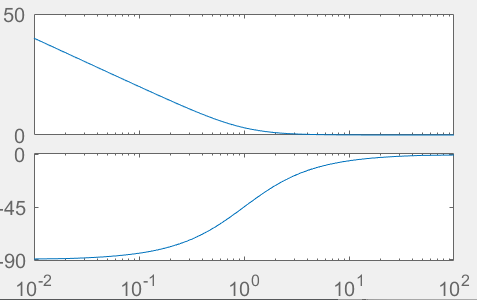
\includegraphics[width = \linewidth]{src/images/PI-controller.png}
        \end{minipage}

    \titel{PD-Controller}
        \begin{minipage}{0.49\linewidth}
            \begin{itemize}
                \item proportional to rate of change of error (reduced overshoot)
                \item pole introduced at $p=0$
                \item zero introduced at $z = -\frac{k_i}{k_p}$
                \item number of asymptotes unchanged
                \item $k_P$ increases:
                \begin{itemize}
                    \item $e_{ss}$ unaffected
                    \item less oscillatory, but potentially slower
                    \item increased sensitivity to noise
                \end{itemize}
            \end{itemize}
        \end{minipage}
        \begin{minipage}{0.49\linewidth}
            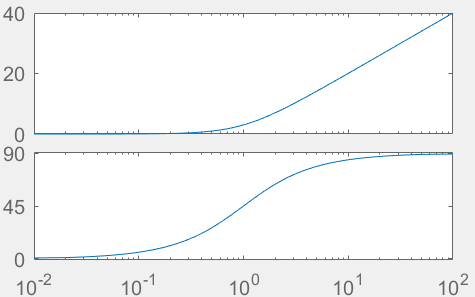
\includegraphics[width = \linewidth]{src/images/PD-controller.png}
        \end{minipage}

    \titel{PID-Controller}
        \begin{scriptsize}
            \begin{align*}
                &C_{\text{PID}}= k_P + \frac{k_I}{s} + k_D \cdot s
                = \frac{k_P \cdot s + k_I + k_D \cdot s^2}{s}
            \end{align*}
        \end{scriptsize}
        \begin{minipage}{0.49\linewidth}
            \begin{scriptsize}
                \begin{align*}
                    &= k_P(1 + \frac{1}{T_I \cdot s} + T_D \cdot s)\\
                    k_P &= \text{Proportional gain}\\
                    k_I &= \text{Integral gain}\\
                    k_D &= \text{Derivative gain}\\
                    T_I &= \text{Integral time constant gain}\\
                    T_D &= \text{Derivative time constant}
                \end{align*}
            \end{scriptsize}
        \end{minipage}
        \begin{minipage}{0.49\linewidth}
            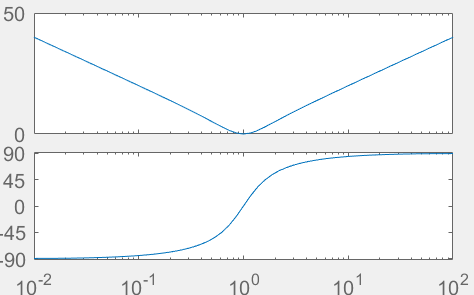
\includegraphics[width = \linewidth]{src/images/PID-controller.png}
        \end{minipage}
